\documentclass[11pt]{article}
\usepackage[margin=1in]{geometry}

\usepackage{amsmath,amssymb}
\usepackage{graphicx}
\usepackage{booktabs}
\usepackage[hidelinks]{hyperref}
\usepackage{array}

\graphicspath{{figures/}}

\setlength{\parindent}{0pt}
\setlength{\parskip}{0.85\baselineskip}

\title{Replication and Robustness Study of Opinion Dynamics on Directed Complex Networks}
\author{Luoxiang Pan, Zhaodong Liu}
\date{\today}

\begin{document}
\maketitle

\begin{abstract}
This project reproduces and stress-tests the stochastic opinion model introduced
by Fraiman, Lin, and Olvera-Cravioto in \emph{Opinion Dynamics on Directed
Complex Networks}~\cite{fraiman2024opinion}.  The source paper studies a
directed network in which each agent combines inbound-neighbor opinions,
attribute-dependent media signals, and a memory term.  We implemented the model
from the published equations, reproduced source-paper Figures~1--7 on directed
Erd\H{o}s--R\'enyi networks, numerically checked the contraction mechanism
behind the stationary limit, and added four robustness experiments involving
topology, selective exposure, bot prevalence, and community structure.  The main
replication is successful at the qualitative level and is close quantitatively
for the central polarization benchmark: in our reproduction of source-paper
Figure~4, the memory case gives
$\mathrm{Var}(R^*)=0.1460$ in the displayed seed, and averaging over ten
independent seeds gives $0.1449\pm0.0006$.  The no-memory case gives
$0.1454\pm0.0006$, close to the corresponding Proposition~4 finite-graph
prediction $0.1459\pm0.0000$.  The variation studies
support the paper's mechanism for selective exposure, but they also clarify its
scope.  Comparable well-connected non-ER networks produce similar outcomes,
whereas sparse or community-aligned networks can substantially alter the
stationary distribution.  Bot experiments mainly shift the regular-agent mean
rather than increasing the separation between ideological groups.  Our critique
therefore is not that the model fails, but that the simulations in the source
paper give less evidence for broad empirical generality than the mathematical
framework itself permits.
\end{abstract}

\tableofcontents

\section{Introduction}

Opinion dynamics models ask how individual-level influence rules produce
population-level outcomes such as agreement, disagreement, or polarization.
This question is especially natural in online social systems.  Interactions on
these systems are often directed: one user can listen to, follow, or amplify
another user without receiving reciprocal influence.  A model that treats
directed edges as a primary feature is therefore better suited to many modern
network settings than an undirected averaging model.

Fraiman, Lin, and Olvera-Cravioto~\cite{fraiman2024opinion} propose such a
model.  Their framework combines three ingredients in a single stochastic
recursion: influence from inbound neighbors, exogenous media signals, and
persistence of the agent's previous opinion.  The model is mathematically
tractable because the update rule is linear, but it is still expressive enough
to represent heterogeneous agents, selective exposure, and stubborn agents.  At
the theoretical level, the paper proves the existence of a stationary opinion
distribution on fixed directed graphs when the media weight is positive.  It
then studies the opinion of a typical vertex in large random directed graphs
through local weak limits.

This paper is a good fit for a replication project in network dynamics for two
reasons.  First, the model is explicitly dynamical: opinions evolve through a
repeated update rule on a graph.  Second, the published conclusions connect
mathematical theory to finite-network simulations, so the computational figures
can be independently rebuilt and inspected.  The paper's figures are also useful
for critical evaluation because they rely almost entirely on directed
Erd\H{o}s--R\'enyi graphs.  This creates a natural question: do the observed
consensus and polarization patterns reflect only the update rule, or do they
also depend on the particular topology used in the simulations?

Our project has four goals.  We first restate the original model and the
theoretical claims that guide the computation.  We then implement the dynamics
from scratch in a modular Python and MATLAB codebase.  Next, we reproduce the
main simulation figures and compare them with the values reported in the paper.
Finally, we run new variation studies to examine whether the paper's
interpretation remains stable when important assumptions are changed.

The repository for the project is public at
\url{https://github.com/PatrickEleeve/Network_Final}.  The remainder of the
paper is organized as follows.  Section~\ref{sec:paper} summarizes the original
mathematical model.  Section~\ref{sec:methods} describes our implementation and
experimental design.  Sections~\ref{sec:replication} and~\ref{sec:variations}
present the replication and robustness results.  Section~\ref{sec:discussion}
gives the scientific interpretation and critique, and
Section~\ref{sec:conclusion} concludes.

\section{Original Paper and Model}
\label{sec:paper}

\subsection{Scientific Question}

The source paper asks how opinions evolve on a directed network when agents are
influenced by neighbors, media, and their own previous state.  The authors are
not only interested in whether the process converges.  They also want to
understand which parameter regimes produce a narrow consensus-like distribution,
which regimes produce separated opinion groups, and how stubborn or artificial
agents affect the population.

\subsection{Opinion Recursion}

Let $R_i^{(k)} \in [-1,1]$ denote the opinion of vertex $i$ at time $k$.  A
directed edge $(j,i)$ means that vertex $i$ listens to vertex $j$.  If $d_i^-$
is the number of inbound neighbors of $i$, and $\ell(i,r)$ is the label of its
$r$th inbound neighbor, the model updates opinions by
\begin{equation}
R_i^{(k+1)}
= \sum_{r=1}^{d_i^-} c(i,r)R_{\ell(i,r)}^{(k)}
  + W_i^{(k)}
  + (1-c-d)R_i^{(k)} .
\label{eq:update}
\end{equation}
The parameter $c$ is the total weight assigned to inbound neighbors, $d$ is the
media weight, and $1-c-d$ is the memory coefficient.  The paper assumes
$c\in[0,1)$, $d\in(0,1]$, and $c+d\leq1$.  For every vertex with at least one
inbound neighbor, the weights satisfy
\[
\sum_{r=1}^{d_i^-} c(i,r)=c.
\]
In our implementation these weights are equal within each inbound neighborhood,
so $c(i,r)=c/d_i^-$ whenever $d_i^->0$.

The external signal is
\begin{equation}
W_i^{(k)}
= q_i\left(c-\sum_{r=1}^{d_i^-}c(i,r)\right)+dZ_i^{(k)} ,
\label{eq:external}
\end{equation}
where $q_i$ is the internal opinion or predisposition of vertex $i$, and
$Z_i^{(k)}\in[-1,1]$ is the media signal.  Equation~\eqref{eq:external} has an
important interpretation.  If a vertex has inbound neighbors, the neighbor
weights sum to $c$, so $W_i^{(k)}=dZ_i^{(k)}$.  If it has no inbound neighbors,
the missing neighbor term is replaced by $cq_i$, making the vertex partly
anchored to its internal opinion.

\subsection{Theoretical Claims Used in the Replication}

The first key theorem is a fixed-graph convergence result.  Define the linear
operator
\[
(\Delta f)(i)=\sum_{r=1}^{d_i^-}c(i,r)f(\ell(i,r))+(1-c-d)f(i).
\]
Because the total non-media weight is at most $1-d$, the operator norm satisfies
$\|\Delta\|_\infty\leq1-d<1$.  The recursion can therefore be written as
$R^{(k+1)}=\Delta R^{(k)}+W^{(k)}$, and the influence of the initial condition
decays geometrically.  This justifies approximating the stationary distribution
with a finite number of iterations, provided $d$ is not too small.

The second key theorem concerns graph sequences.  Under a strong local coupling
assumption, the opinion of a uniformly selected vertex in a large directed
random graph converges to the stationary opinion at the root of the local weak
limit.  In tree-like cases this limit can be described through branching
recursions.  This result explains why simulations on large sparse random graphs
can approximate the distribution of a typical individual, not only the behavior
of one particular vertex.

The paper also gives moment formulas in the no-memory case $c+d=1$.  These
formulas are useful for interpreting the polarization experiment.  When media
signals depend strongly on $q_i$, the conditional mean
$\mathbb{E}[Z_i\mid q_i]$ differs across groups; the law of total variance then
predicts a stationary distribution with separated conditional centers.  This is
the mathematical mechanism behind source-paper Figure~4.

\section{Replication Design and Implementation}
\label{sec:methods}

\subsection{Codebase}

The implementation is organized around the structure of
Equations~\eqref{eq:update} and~\eqref{eq:external}.  The directory
\texttt{src/} contains reusable modules, while \texttt{scripts/} contains
figure-level entry points.  The same dynamics code is used for all baseline and
variation experiments.

\texttt{graph\_construction.py} builds directed networks and returns a sparse
matrix $A$ with entries $A[i,j]$ equal to the weight that vertex $i$ assigns to
inbound neighbor $j$.  Thus the neighbor term is computed as $A R^{(k)}$.  The
module includes directed Erd\H{o}s--R\'enyi graphs, a bot-augmented graph for
source-paper Figure~5, a directed power-law configuration model for the topology
variation, and a directed stochastic block model for the community experiment.

\texttt{attributes.py} samples vertex attributes.  Source-paper
Figures~1--3 use $Q_i\sim U(-1,1)$; source-paper Figures~4--7 use
$Q_i\in\{-1,+1\}$ with equal probability.
For the bot experiment, bot vertices are assigned $Q_i=+1$ and a stubborn flag
$S_i=1$.  \texttt{signals.py} implements the media distributions $Z_i^{(k)}$
for each scenario and then converts them into $W_i^{(k)}$ using
Equation~\eqref{eq:external}.  \texttt{dynamics.py} contains the one-step update
and the simulation routine \texttt{run\_to\_stationarity}.  Finally,
\texttt{validation.py} computes empirical moments and performs the coupled-chain
test for Theorem~1.

The paper PDF does not provide a code repository or fixed random seeds for the
figures.  We therefore implemented the model independently from the equations
and documented the additional choices in the scripts.  All reported figures can
be regenerated from the repository using the commands listed in the appendix.

\subsection{Simulation Parameters}

The baseline experiments use the same finite-network scale as the paper:
$n=1000$ and directed Erd\H{o}s--R\'enyi edge probability $p=0.03$, except for
source-paper Figure~5, where the graph contains $800$ regular vertices and
$200$ bots.  The initial opinions are sampled from $\{-1,+1\}$, following the
paper's simulation description.  Table~\ref{tab:baseline-params} summarizes the
main parameter choices.

\begin{table}[t]
\centering
\resizebox{\textwidth}{!}{%
\begin{tabular}{lllll}
\toprule
Scenario & Memory case $(c,d)$ & No-memory case $(c,d)$ & Signal $Z$ & Iterations \\
\midrule
Source Fig. 1 & $(0.001,0.300)$ & $(0.003322,0.996678)$ & $U(-0.03,0.03)$ & 500 \\
Source Fig. 2 & $(0.500,0.001)$ & $(0.998004,0.001996)$ & $\{-1,+1\}$ & 16000 max \\
Source Fig. 3 & $(0.500,0.001)$ & $(0.998004,0.001996)$ & $-1+2\mathrm{Beta}(1,8)$ & 16000 max \\
Source Fig. 4 & $(0.500,0.450)$ & $(0.5263,0.4737)$ & selective exposure & 200 \\
Source Fig. 5 & $(0.500,0.450)$ & $(0.5263,0.4737)$ & selective exposure + bots & 200 \\
Source Fig. 6 & $(0.300,0.200)$ & $(0.600,0.400)$ & $U(-1,1)$ & 300 \\
Source Fig. 7 & $(0.300,0.200)$ & $(0.600,0.400)$ & $U(-1,1)$ & 50 \\
\bottomrule
\end{tabular}
}
\caption{Baseline simulation settings.  The no-memory cases rescale $c$ and
$d$ proportionally so that $c+d=1$, matching the comparison used in the source
paper.}
\label{tab:baseline-params}
\end{table}

For source-paper Figures~4 and~5, selective exposure is implemented as
$Z_i\sim -1+2\mathrm{Beta}(8,1)$ when $Q_i=+1$ and
$Z_i\sim -1+2\mathrm{Beta}(1,8)$ when $Q_i=-1$.  Bots in source-paper
Figure~5 broadcast $Z_i=+1$ and receive no inbound influence.  The iteration
counts are larger than the contraction estimate requires in the $d=0.45$ and
$d=0.2$ cases, but we used conservative horizons to avoid confusing transient
behavior with the stationary distribution.

For clarity, Table~\ref{tab:figure-map} separates the figure numbering in this
paper from the figure numbering in the source paper.  The validation plot is
our own diagnostic figure; the next seven figures reproduce source-paper
Figures~1--7.

\begin{table}[t]
\centering
\scriptsize
\begin{tabular}{p{0.16\textwidth}p{0.29\textwidth}p{0.45\textwidth}}
\toprule
This paper & Image file & Meaning \\
\midrule
Fig.~\ref{fig:theorem1-convergence} & \path|theorem1_convergence.png| & Theorem~1 contraction diagnostic \\
Fig.~\ref{fig:fig1-replication} & \path|fig1_replication.png| & Source-paper Figure~1 replication \\
Fig.~\ref{fig:fig2-replication} & \path|fig2_replication.png| & Source-paper Figure~2 replication \\
Fig.~\ref{fig:fig3-replication} & \path|fig3_replication.png| & Source-paper Figure~3 replication \\
Fig.~\ref{fig:fig4-replication} & \path|fig4_replication.png| & Source-paper Figure~4 replication \\
Fig.~\ref{fig:fig5-replication} & \path|fig5_replication.png| & Source-paper Figure~5 replication \\
Fig.~\ref{fig:fig6-replication} & \path|fig6_replication.png| & Source-paper Figure~6 replication \\
Fig.~\ref{fig:fig7-replication} & \path|fig7_replication.png| & Source-paper Figure~7 replication \\
Fig.~\ref{fig:variation1-topology} & \path|variation1_topology.png| & New topology robustness study \\
Fig.~\ref{fig:variation2-beta} & \path|variation2_beta_scan.png| & New selective-exposure scan \\
Fig.~\ref{fig:variation3-bots} & \path|variation3_bot_scan.png| & New bot-prevalence scan \\
Fig.~\ref{fig:variation4-community} & \path|variation4_community.png| & New community-structure study \\
\bottomrule
\end{tabular}
\caption{Figure correspondence audit.  ``Source-paper Figure'' refers to the
numbering in Fraiman, Lin, and Olvera-Cravioto~\cite{fraiman2024opinion};
``This paper'' refers to the automatic figure numbering in this report.}
\label{tab:figure-map}
\end{table}

\subsection{Evaluation Criteria}

We evaluated the replication in two ways.  The first criterion is visual and
qualitative: the reproduced histograms and trajectories should have the same
shape and interpretation as the published figures.  The second criterion is
quantitative: where the paper reports or implies summary values, we compare
empirical means, variances, conditional means, and conditional variances.

We also verified the contraction claim behind Theorem~1.  Two chains with
different initial conditions were driven by the same media-signal realization,
so their difference followed $\Delta$ without additional noise.  As shown in
Figure~\ref{fig:theorem1-convergence}, all tested cases stayed within the
theoretical bound $1-d$.  The empirical rates were $0.9459$, $0.7896$,
$0.5250$, and $0.1306$ for $d=0.05$, $0.20$, $0.45$, and $0.80$ respectively,
all below the corresponding bounds.

\begin{figure}[t]
    \centering
    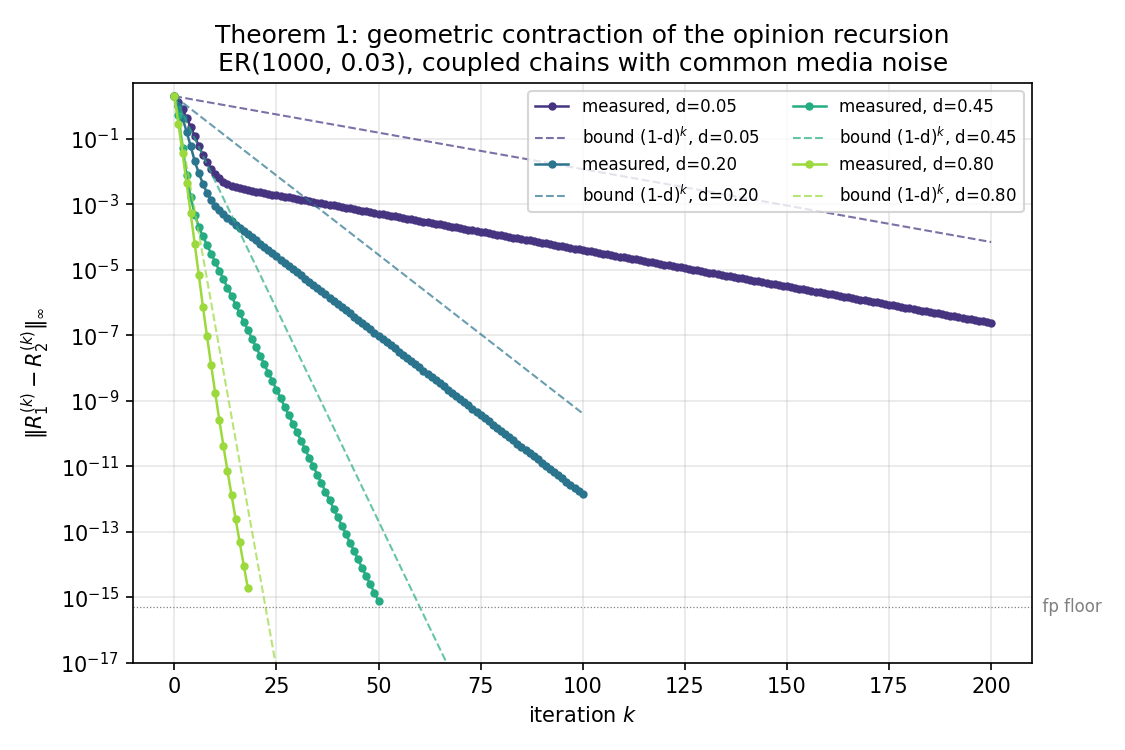
\includegraphics[width=0.78\textwidth]{theorem1_convergence}
    \caption{Numerical validation of Theorem~1.  Coupled chains with common
    media noise contract at rates below the theoretical bound $1-d$.}
    \label{fig:theorem1-convergence}
\end{figure}

\section{Replication Results}
\label{sec:replication}

\subsection{Source-Paper Figures 1--3: Consensus-Type Outcomes}

Source-paper Figures~1--3 test regimes in which the stationary opinion
distribution is expected to be narrow.  Our reproductions match this qualitative
conclusion.  In the source-paper Figure~1 setup, where the media signal has
very small variance, both the memory and no-memory cases concentrate near zero.
The empirical variances are
$5.0\times10^{-5}$ and $2.98\times10^{-4}$, respectively.  The small difference
between the panels is consistent with the stronger direct media weight in the
no-memory rescaling.

\begin{figure}[t]
    \centering
    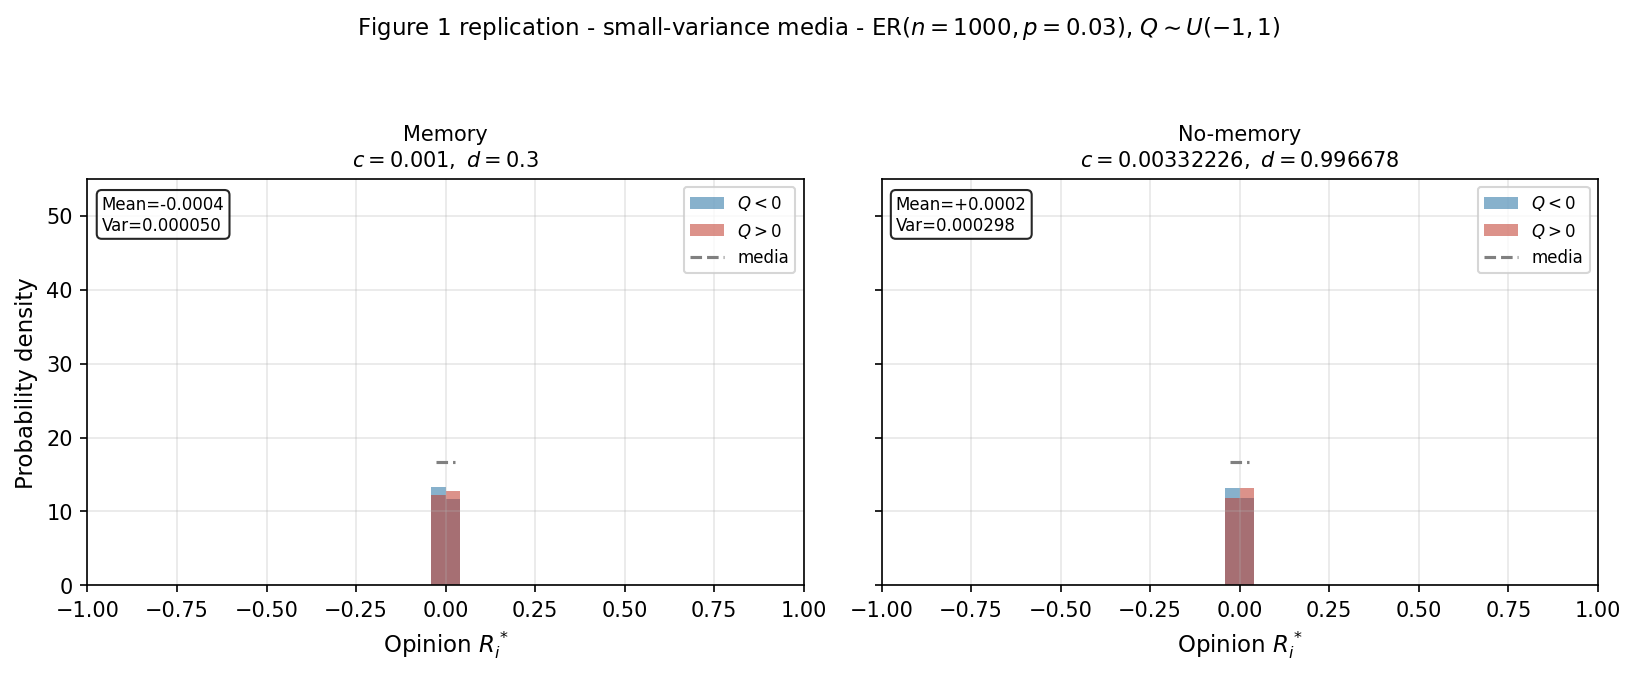
\includegraphics[width=0.75\textwidth]{fig1_replication}
    \caption{Replication of source-paper Figure~1.  Low-variance media
    produces a narrow stationary distribution centered near zero.}
    \label{fig:fig1-replication}
\end{figure}

The source-paper Figure~2 setup uses a highly variable media signal taking
values in $\{-1,+1\}$, but the media weight is only $d=0.001$ in the memory
case.  Neighbor averaging then dominates the update, and the distribution again
collapses tightly around zero.  Our measured variances are
$1.0\times10^{-6}$ for the memory case and $4.0\times10^{-6}$ for the
no-memory case.

\begin{figure}[t]
    \centering
    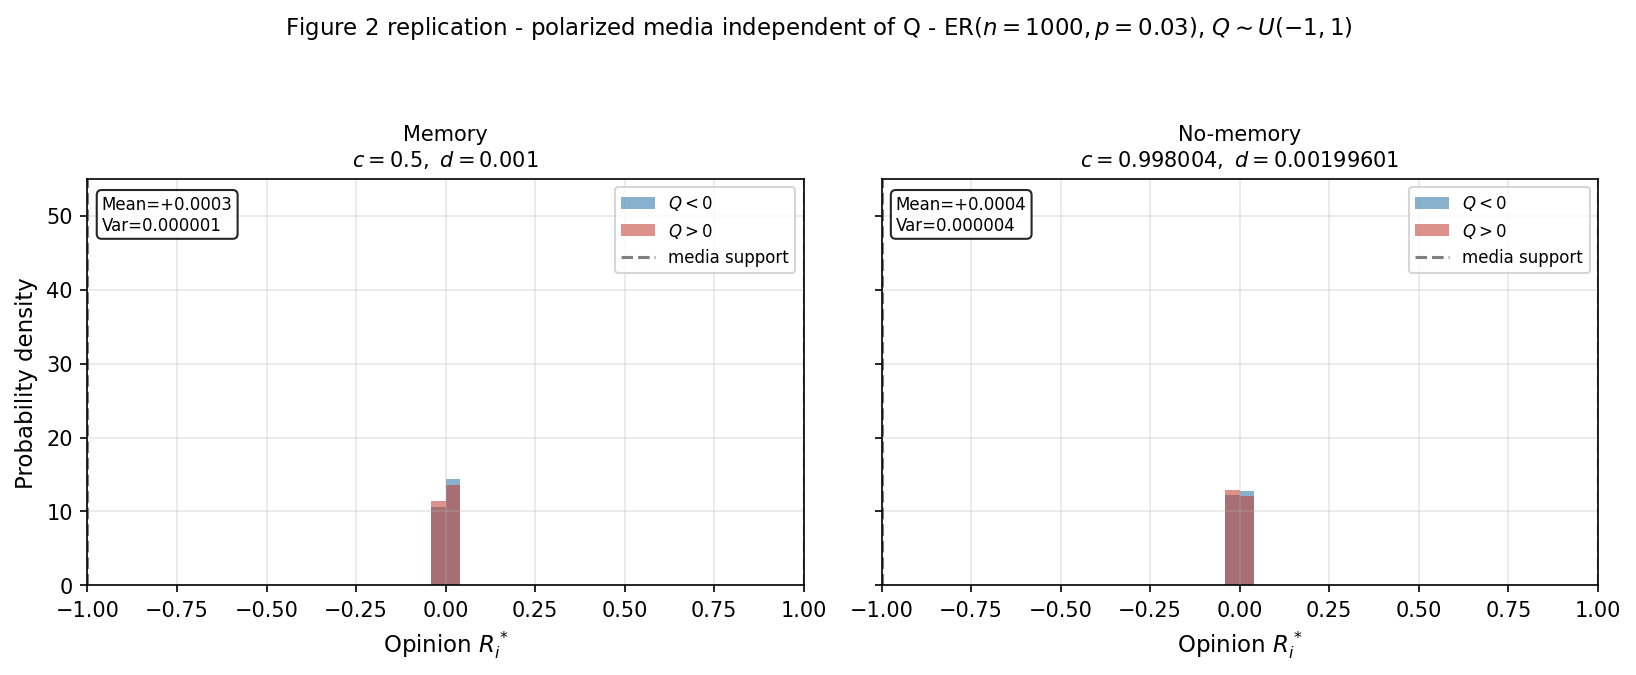
\includegraphics[width=0.75\textwidth]{fig2_replication}
    \caption{Replication of source-paper Figure~2.  Even with binary media
    signals, the small media weight and network averaging lead to near
    consensus.}
    \label{fig:fig2-replication}
\end{figure}

The source-paper Figure~3 setup changes the media distribution to a shifted
$\mathrm{Beta}(1,8)$, which has negative mean.  The population still reaches a
tight distribution, but its center moves to approximately $-0.778$.  Our memory
and no-memory runs produce means $-0.7776$ and $-0.7777$, with variance
essentially zero at the displayed precision.

\begin{figure}[t]
    \centering
    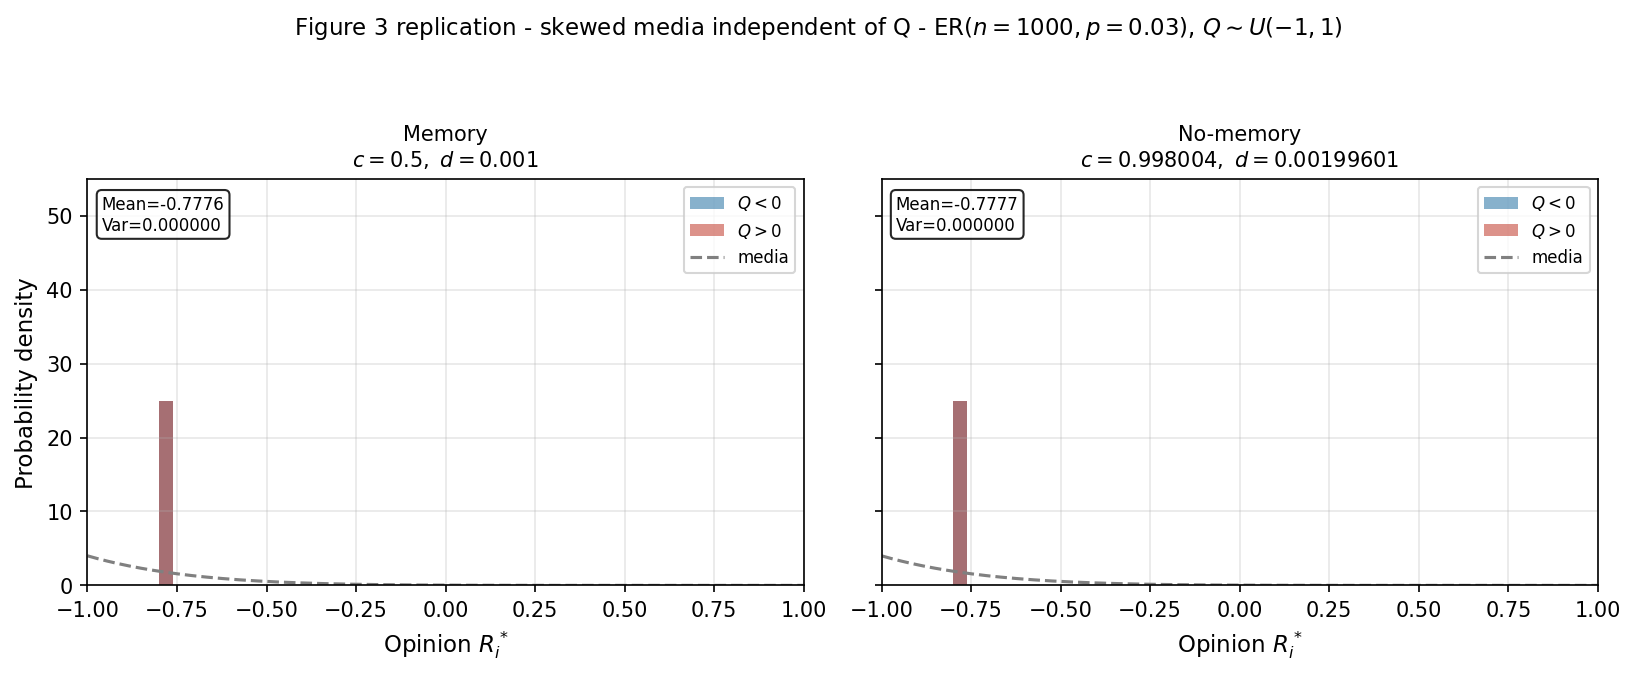
\includegraphics[width=0.75\textwidth]{fig3_replication}
    \caption{Replication of source-paper Figure~3.  A biased media distribution
    moves the consensus point away from zero while keeping the population
    tightly concentrated.}
    \label{fig:fig3-replication}
\end{figure}

\subsection{Source-Paper Figure 4: Polarization from Selective Exposure}

The source paper's Figure~4 is the strongest quantitative match in our
replication.  This scenario links the media distribution to the internal opinion
$Q_i$, so the two groups receive systematically different signals.  In the
memory case, we obtain $\mathrm{Var}(R^*)=0.1460$ in the displayed seed.  The
source paper reports a nearby Figure~4 benchmark of approximately $0.1484$.
This value should be read as a source-paper numerical reference, not as a
direct Proposition~4 prediction for the memory case, because Proposition~4
assumes $c+d=1$.  The conditional means are
$\mathbb{E}[R^*\mid Q=+1]=0.3738$ and
$\mathbb{E}[R^*\mid Q=-1]=-0.3646$, compared with the paper's reference values
near $0.3684$ and $-0.3684$.  Conditional variances are also close:
$0.0092$ and $0.0103$, relative to the reported value near $0.0095$.

The no-memory panel is similarly close, with $\mathrm{Var}(R^*)=0.1451$ and
conditional means $0.3679$ and $-0.3627$.  For the realized no-memory graph,
$\rho_2=n^{-1}\sum_i\sum_j A_{ij}^2=0.00958$, and the Proposition~4
finite-graph prediction is $\mathrm{Var}(R^*)=0.1460$.  Across ten independent
graph, attribute, and dynamics seeds, the memory variance is
$0.1449\pm0.0006$ and the no-memory variance is $0.1454\pm0.0006$; the
no-memory Proposition~4 prediction is $0.1459\pm0.0000$.  These results support
the paper's main polarization mechanism: when $d$ is large enough and
$\mathbb{E}[Z\mid Q]$ differs sharply across groups, the stationary distribution
splits into two clusters instead of collapsing to one consensus point.

\begin{figure}[t]
    \centering
    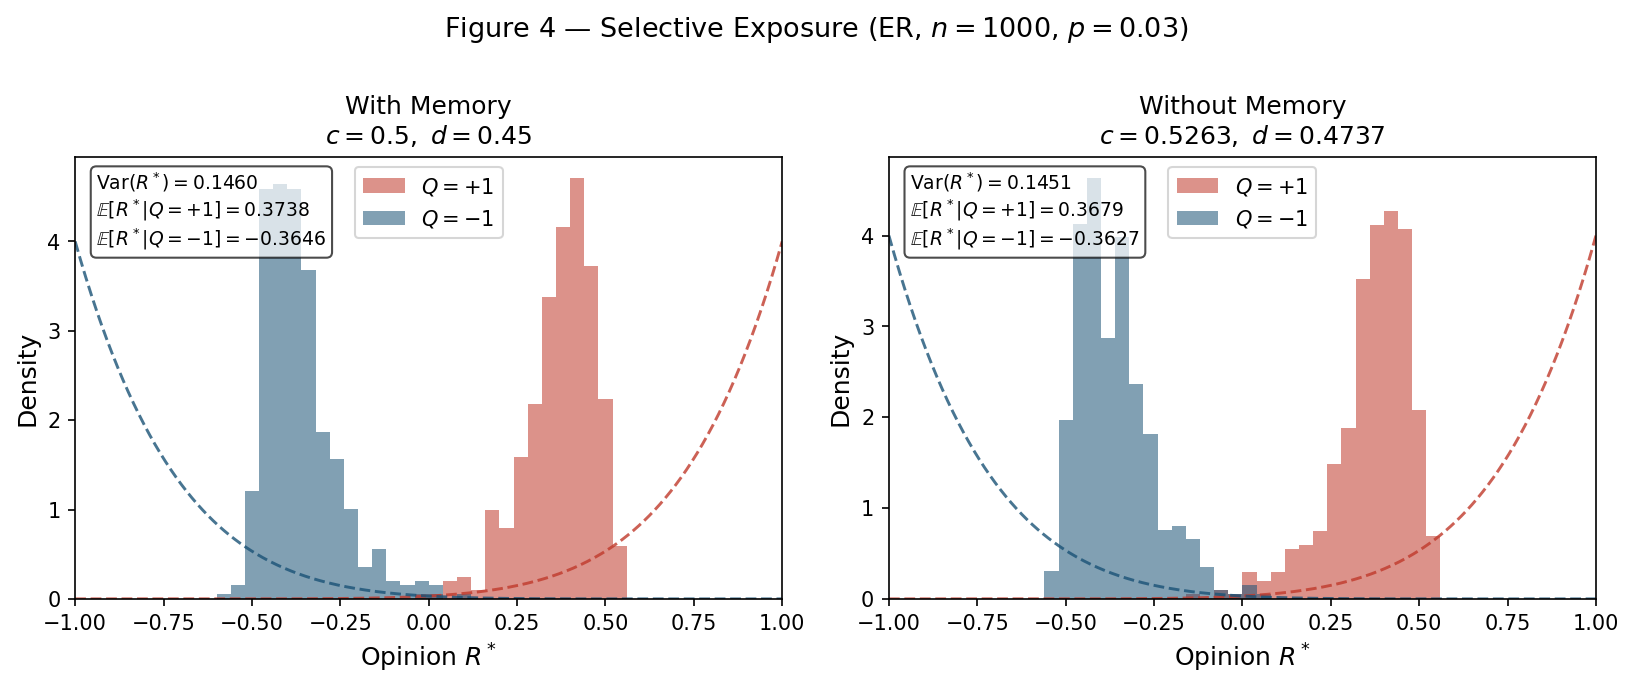
\includegraphics[width=0.85\textwidth]{fig4_replication}
    \caption{Replication of source-paper Figure~4.  Attribute-dependent media
    exposure produces a bimodal stationary distribution with group centers close
    to the values reported in the source paper.}
    \label{fig:fig4-replication}
\end{figure}

\subsection{Source-Paper Figure 5: Stubborn Bots}

The source-paper Figure~5 setup adds $200$ bots to $800$ regular agents.  Bots
have zero in-degree, hold $Q=+1$, and broadcast $Z=+1$.  Our reproduction
confirms that bots push regular opinions in the positive direction.  In the
memory case, the regular-agent mean is $0.2038$, while bot opinions remain at
$+1$.  The regular conditional means are $0.5596$ for $Q=+1$ and $-0.1740$ for
$Q=-1$.

This result is better interpreted as a distribution shift than as a new form of
polarization.  The negative group moves toward the bots, and the positive group
also moves upward; the whole regular-agent distribution is displaced.  The
source paper itself notes that bots are less effective at polarizing when they
cannot target individuals by internal opinion.  Our reproduction supports that
more careful interpretation.

\begin{figure}[t]
    \centering
    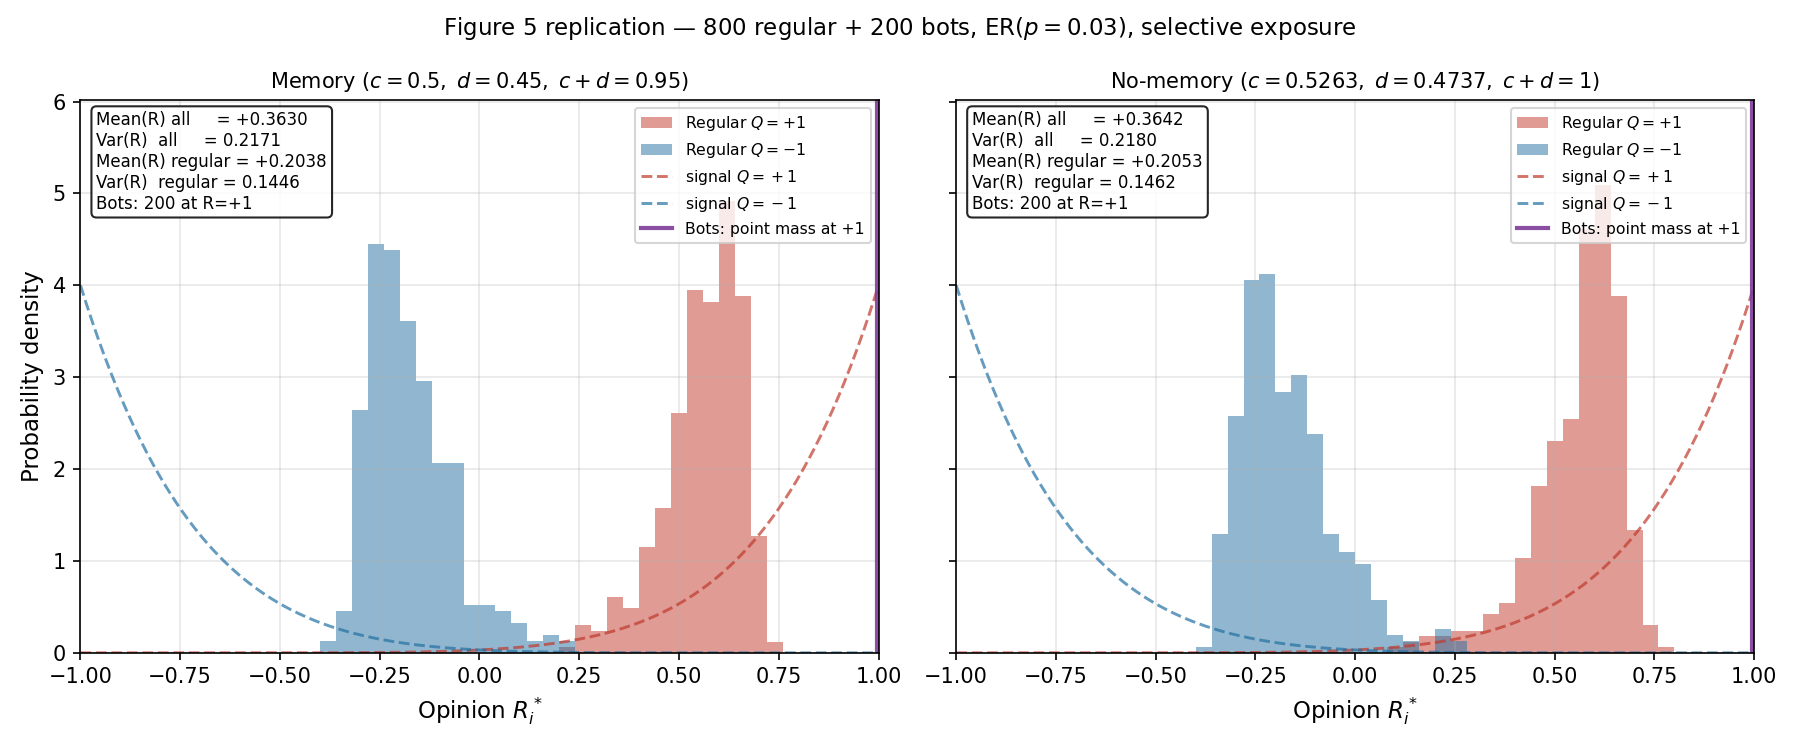
\includegraphics[width=0.85\textwidth]{fig5_replication}
    \caption{Replication of source-paper Figure~5.  Positive bots shift regular
    opinions toward $+1$, but the effect is primarily a mean shift rather than a
    large increase in the two-group gap.}
    \label{fig:fig5-replication}
\end{figure}

\subsection{Source-Paper Figures 6--7: Memory and Trajectories}

Source-paper Figure~6 compares a memory process with $(c,d)=(0.3,0.2)$ to a
no-memory process with the same neighbor/media ratio, $(c,d)=(0.6,0.4)$.  The
reproduced statistics clearly support the paper's variance-compression claim.
The memory case has variance $0.018821$, while the no-memory case has variance
$0.053627$, a reduction of about $64.9\%$.

\begin{figure}[t]
    \centering
    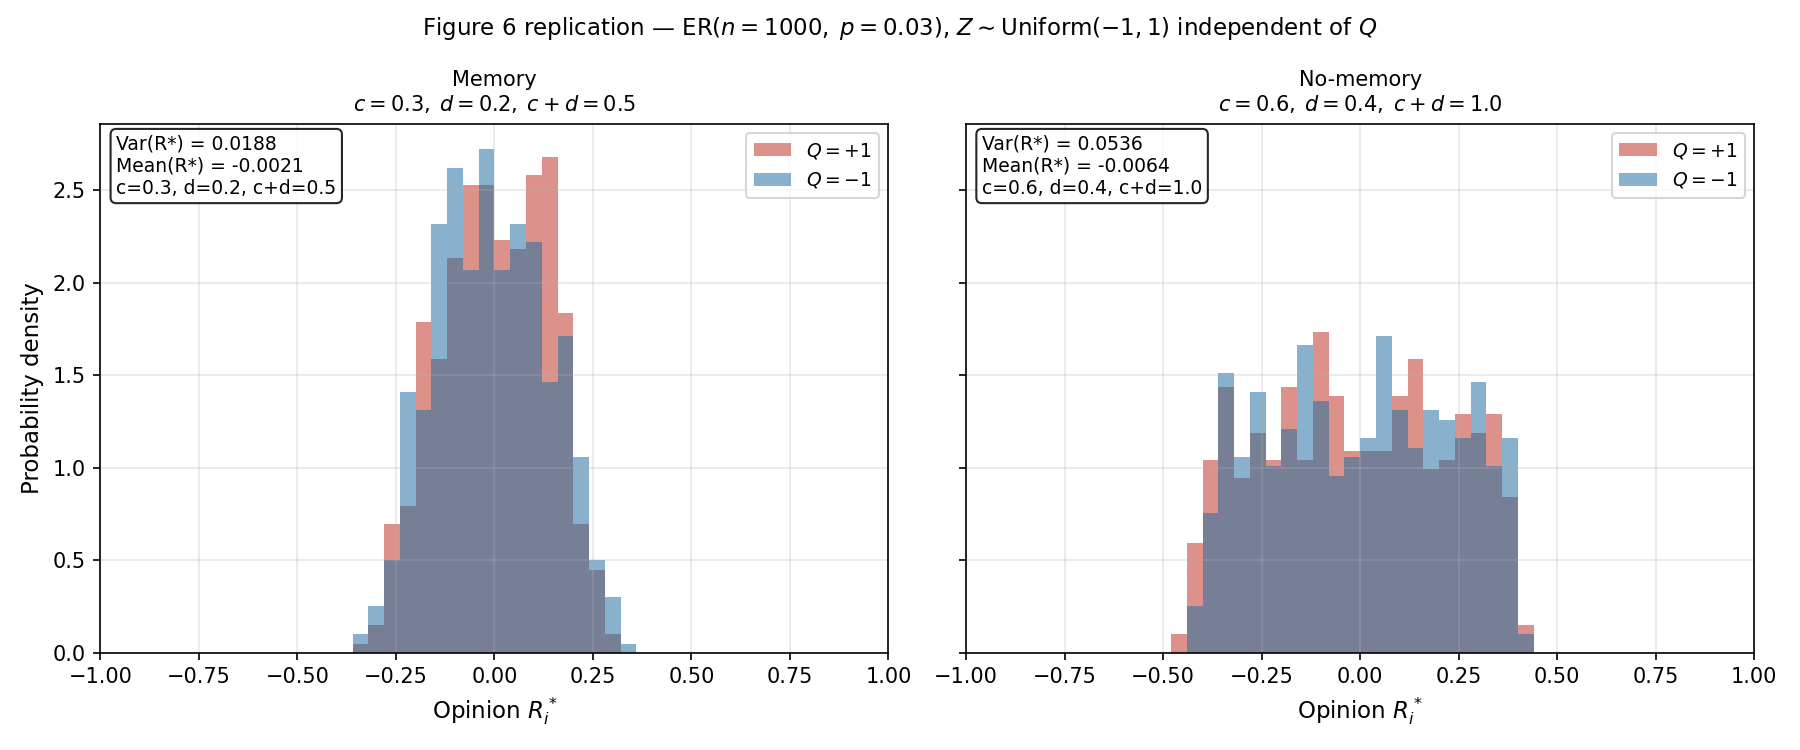
\includegraphics[width=0.85\textwidth]{fig6_replication}
    \caption{Replication of source-paper Figure~6.  The memory term
    substantially reduces stationary variance relative to the proportionally
    equivalent no-memory dynamics.}
    \label{fig:fig6-replication}
\end{figure}

Source-paper Figure~7 shows individual trajectories over time.  Because this
figure tracks only two vertices for $50$ iterations, it is more sensitive to
random realizations than the histogram figures.  Nevertheless, the main
qualitative pattern is reproduced: memory smooths short-run fluctuations.  We
measured average step-to-step roughness of $0.1179$ in the memory panel and
$0.2945$ in the no-memory panel, giving a ratio of about $0.400$.

\begin{figure}[t]
    \centering
    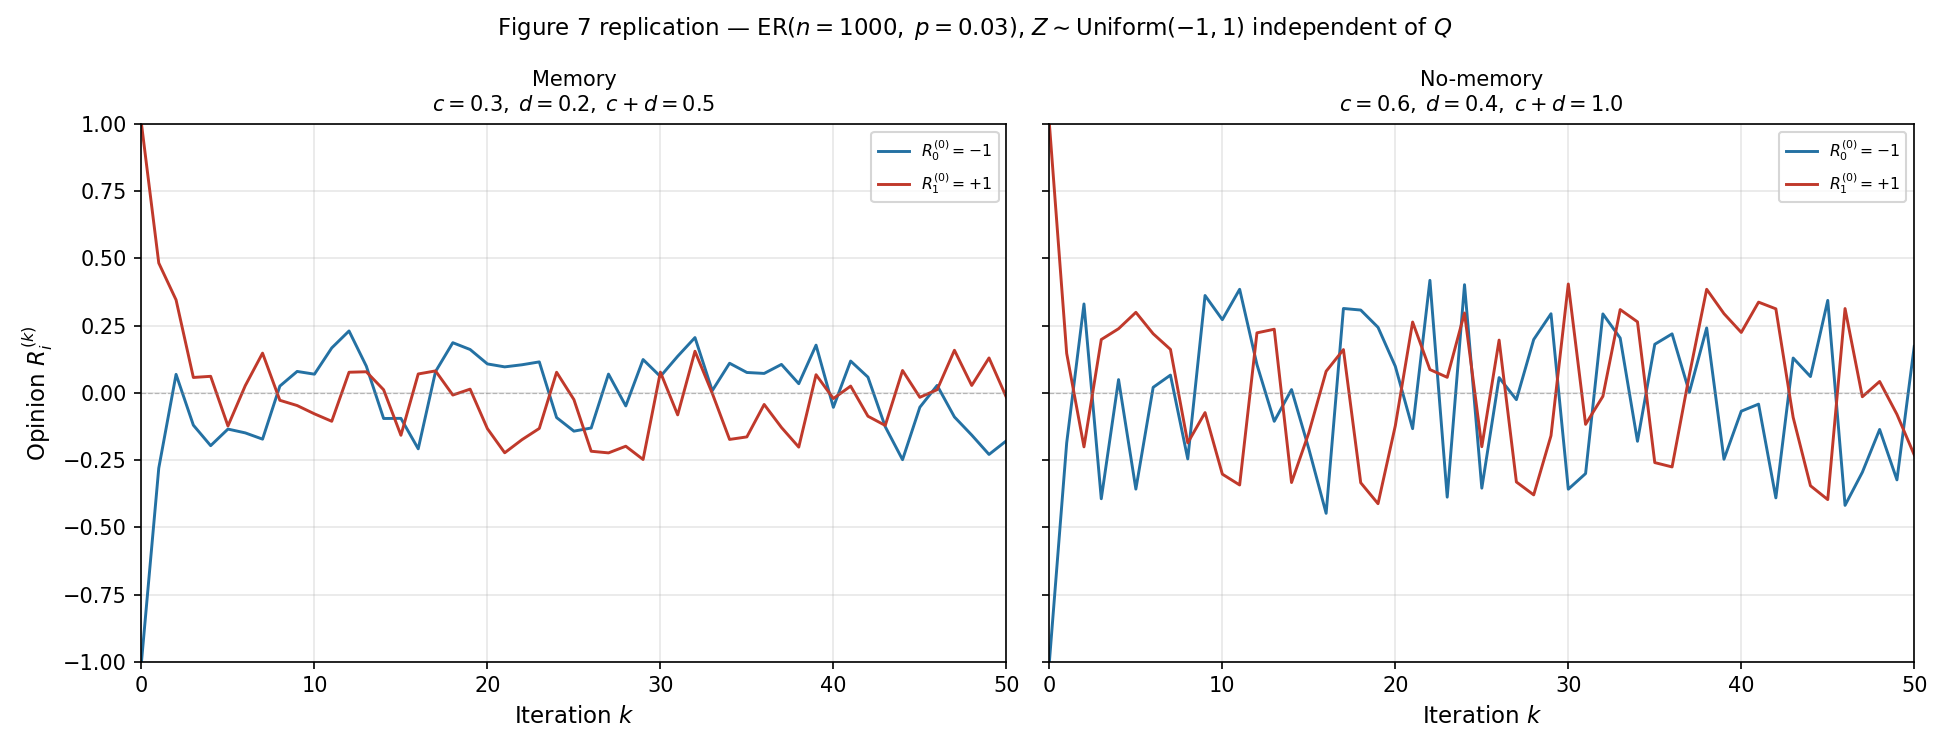
\includegraphics[width=0.85\textwidth]{fig7_replication}
    \caption{Replication of source-paper Figure~7.  Recorded trajectories are
    visibly smoother with memory than without memory.}
    \label{fig:fig7-replication}
\end{figure}

\subsection{Replication Summary}

The replication is strongest for source-paper Figures~1--4 and~6.  These
figures depend on distributional summaries over many vertices, so their
finite-sample behavior is relatively stable.  Source-paper Figure~4 is the most
important success because it reproduces the paper's central selective-exposure
result both visually and numerically.  Source-paper Figures~5 and~7 are still
qualitatively consistent with the source paper, but they are more sensitive to
choices that are not fully
specified in the article, such as the exact graph realization, random seed,
tracked vertices, and plotting convention.  Overall, the implementation
recovers the paper's main computational claims while making the role of
underspecified simulation choices visible.

\section{Variation Studies}
\label{sec:variations}

\subsection{Variation 1: Topology Sensitivity}

The first variation tests whether the source-paper Figure~4 polarization result
is specific to directed Erd\H{o}s--R\'enyi graphs.  We kept the
selective-exposure dynamics fixed at $(c,d)=(0.5,0.45)$ and compared ER graphs
with several directed power-law configuration-model graphs.  We recorded degree
diagnostics because changes in mean degree and low-degree mass can affect the
recursion directly.

The result is nuanced.  Well-connected power-law graphs with mean in-degree
comparable to the ER baseline produce almost the same opinion distribution.  For
example, a power-law graph with $\alpha=2.5$ and $d_{\min}=12$ has variance
$0.1447$, very close to the ER value $0.1460$.  By contrast, sparse graphs have
larger dispersion.  The sparse ER graph with mean in-degree $2.04$ has variance
$0.2763$, and the low-degree power-law graph with mean in-degree $1.81$ has
variance $0.1929$.

\begin{figure}[t]
    \centering
    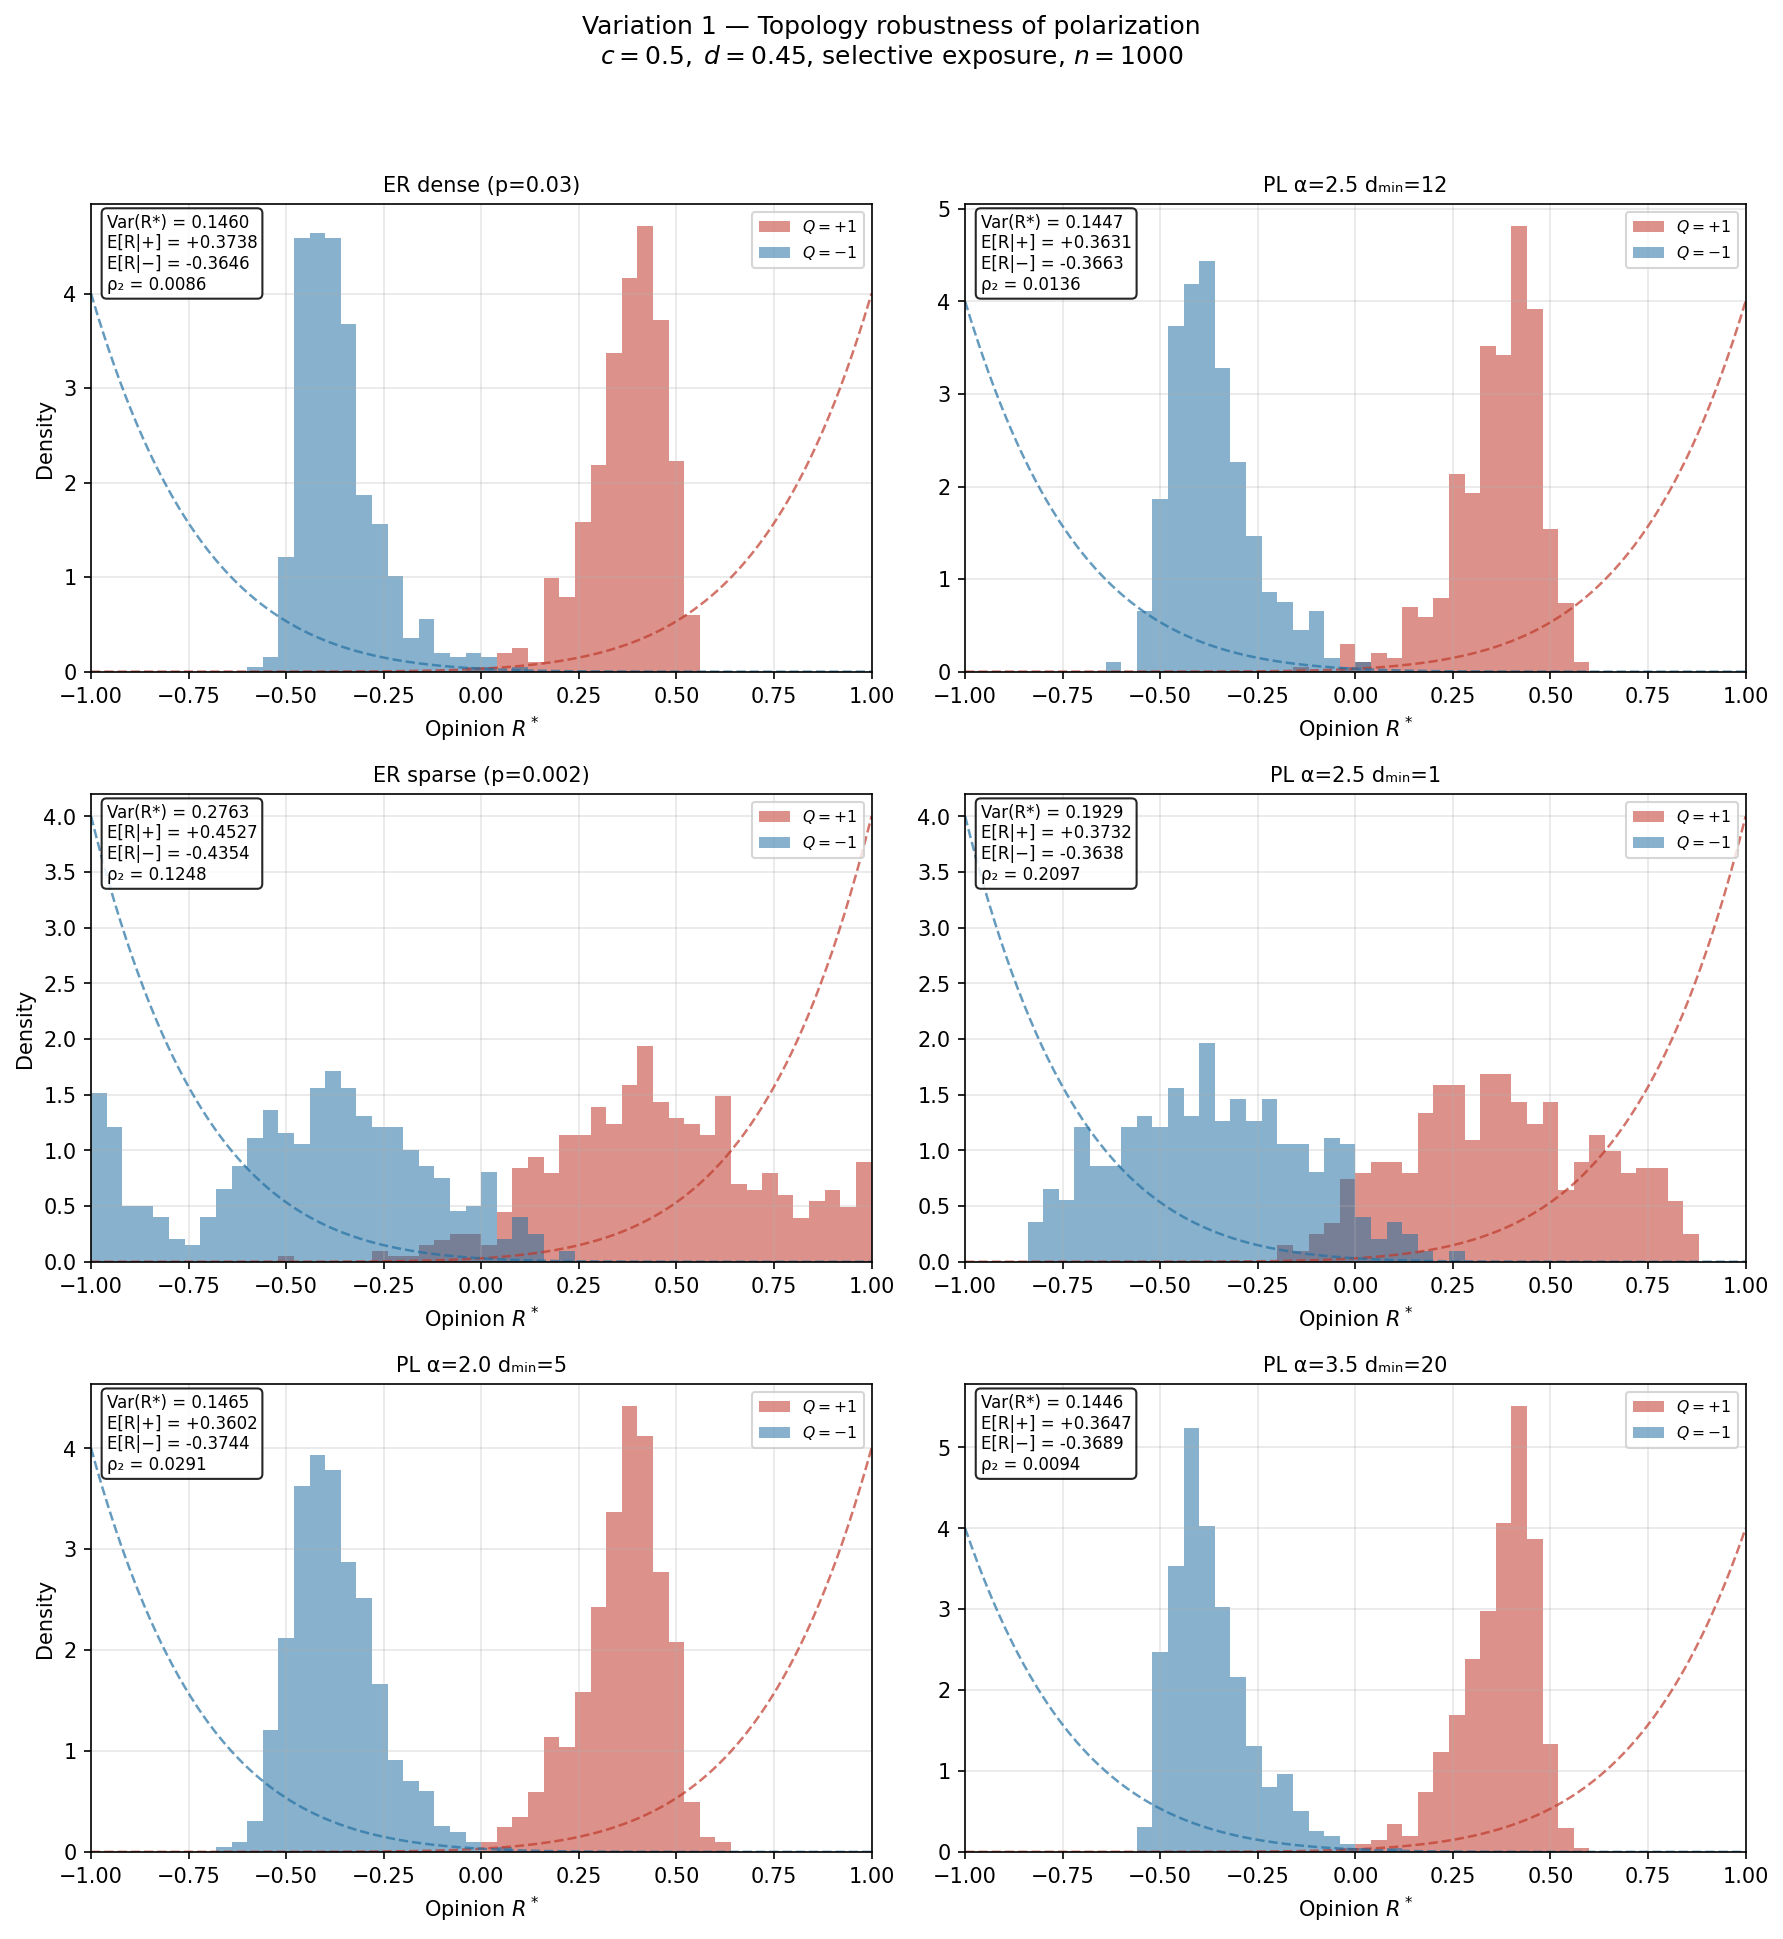
\includegraphics[width=0.9\textwidth]{variation1_topology}
    \caption{Variation~1: topology sensitivity.  Higher-degree power-law graphs
    with comparable degree scale resemble the ER baseline, while sparse or
    low-degree networks produce larger dispersion.}
    \label{fig:variation1-topology}
\end{figure}

This weakens a simple criticism that ``power-law topology breaks the result.''
It does not.  A more defensible critique is that the published simulations do
not explore how degree scale, zero-in-degree vertices, and local heterogeneity
interact with the theory.  The theorem covers a broad class of graph sequences,
but the finite-network evidence in the paper is concentrated on one topology.

\subsection{Variation 2: Selective-Exposure Strength}

The second variation varies the Beta shape parameter in the selective-exposure
signal.  For $Q=+1$, we used $Z=-1+2\mathrm{Beta}(b,1)$; for $Q=-1$, we used
$Z=-1+2\mathrm{Beta}(1,b)$.  Source-paper Figure~4 corresponds to $b=8$.

The polarization gap increases smoothly with $b$.  At $b=1$, media exposure is
approximately symmetric and the conditional mean gap is only $0.0112$.  At
$b=1.5$, the gap is already $0.2140$; at $b=3$, it rises to $0.4716$; and at
$b=8$, it reaches $0.7310$.  The overall variance follows the same broad trend,
moving from $0.0701$ at $b=1$ to $0.1425$ at $b=8$.

\begin{figure}[t]
    \centering
    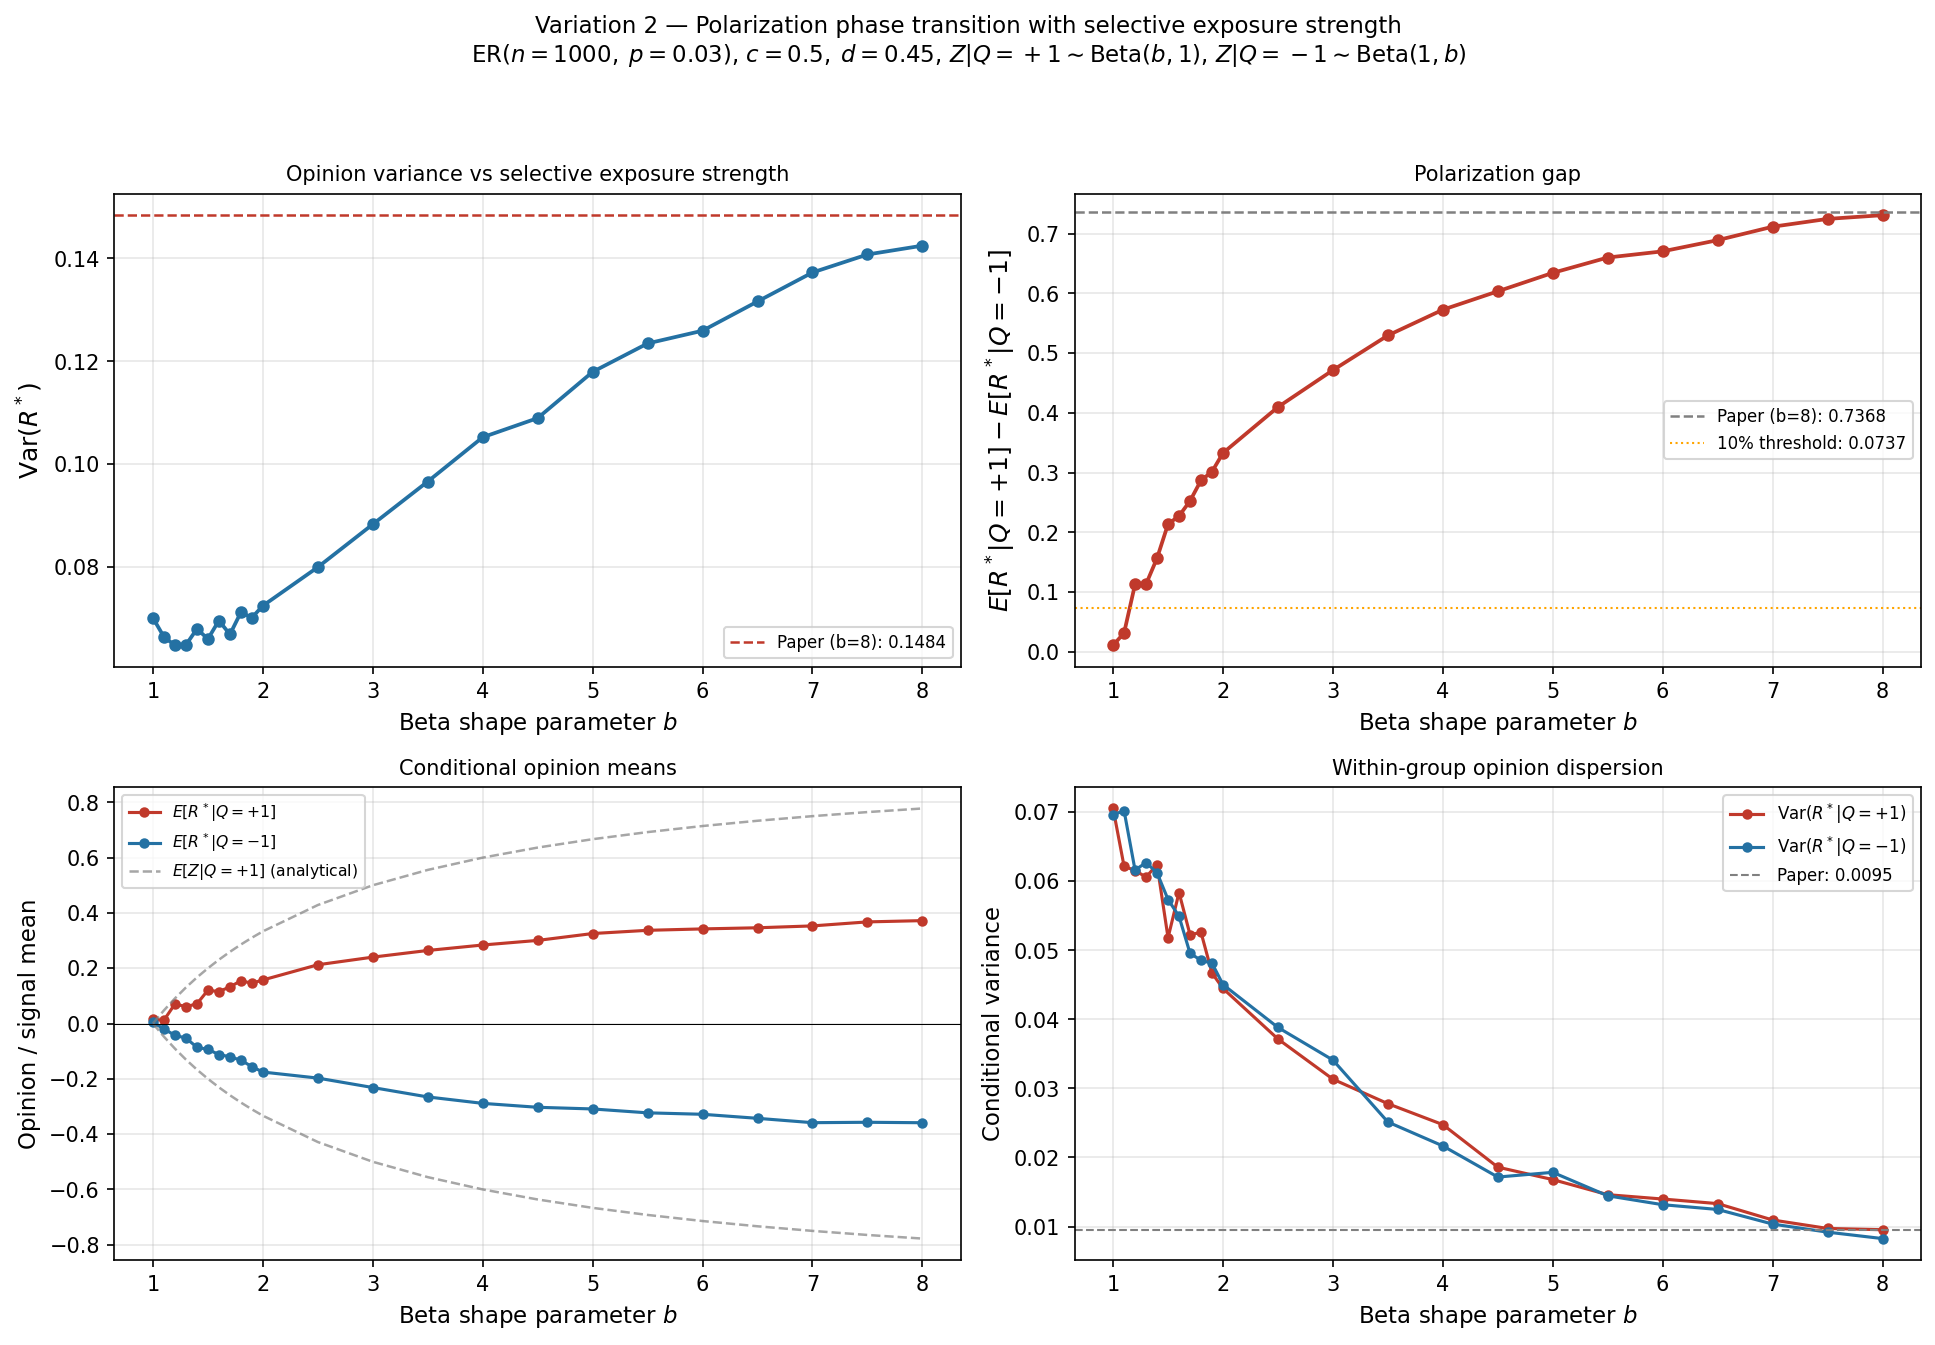
\includegraphics[width=0.85\textwidth]{variation2_beta_scan}
    \caption{Variation~2: selective-exposure strength.  Increasing the Beta
    asymmetry continuously widens the conditional mean gap.}
    \label{fig:variation2-beta}
\end{figure}

This experiment supports the paper's mechanism but adds information that the
single published parameter point cannot show.  Polarization does not appear
only at the extreme $b=8$ setting.  It grows continuously as the conditional
media means separate.

\subsection{Variation 3: Bot Influence}

The third variation scans bot prevalence from $0\%$ to $50\%$ of the network
and compares asymmetric bots with balanced bots.  The key metric is the
regular-agent conditional mean gap
$\mathbb{E}[R^*\mid Q=+1]-\mathbb{E}[R^*\mid Q=-1]$, not merely the population
mean.

Asymmetric positive bots create a strong mean shift.  The regular-agent mean
moves from $0.0026$ with no bots to $0.3722$ at $50\%$ bots.  The conditional
gap, however, barely changes: it is $0.7387$ with no bots and $0.7439$ at
$50\%$ bots, an increase of only about $0.7\%$.  Balanced bots keep the regular
mean close to zero and also leave the conditional gap almost unchanged.

\begin{figure}[t]
    \centering
    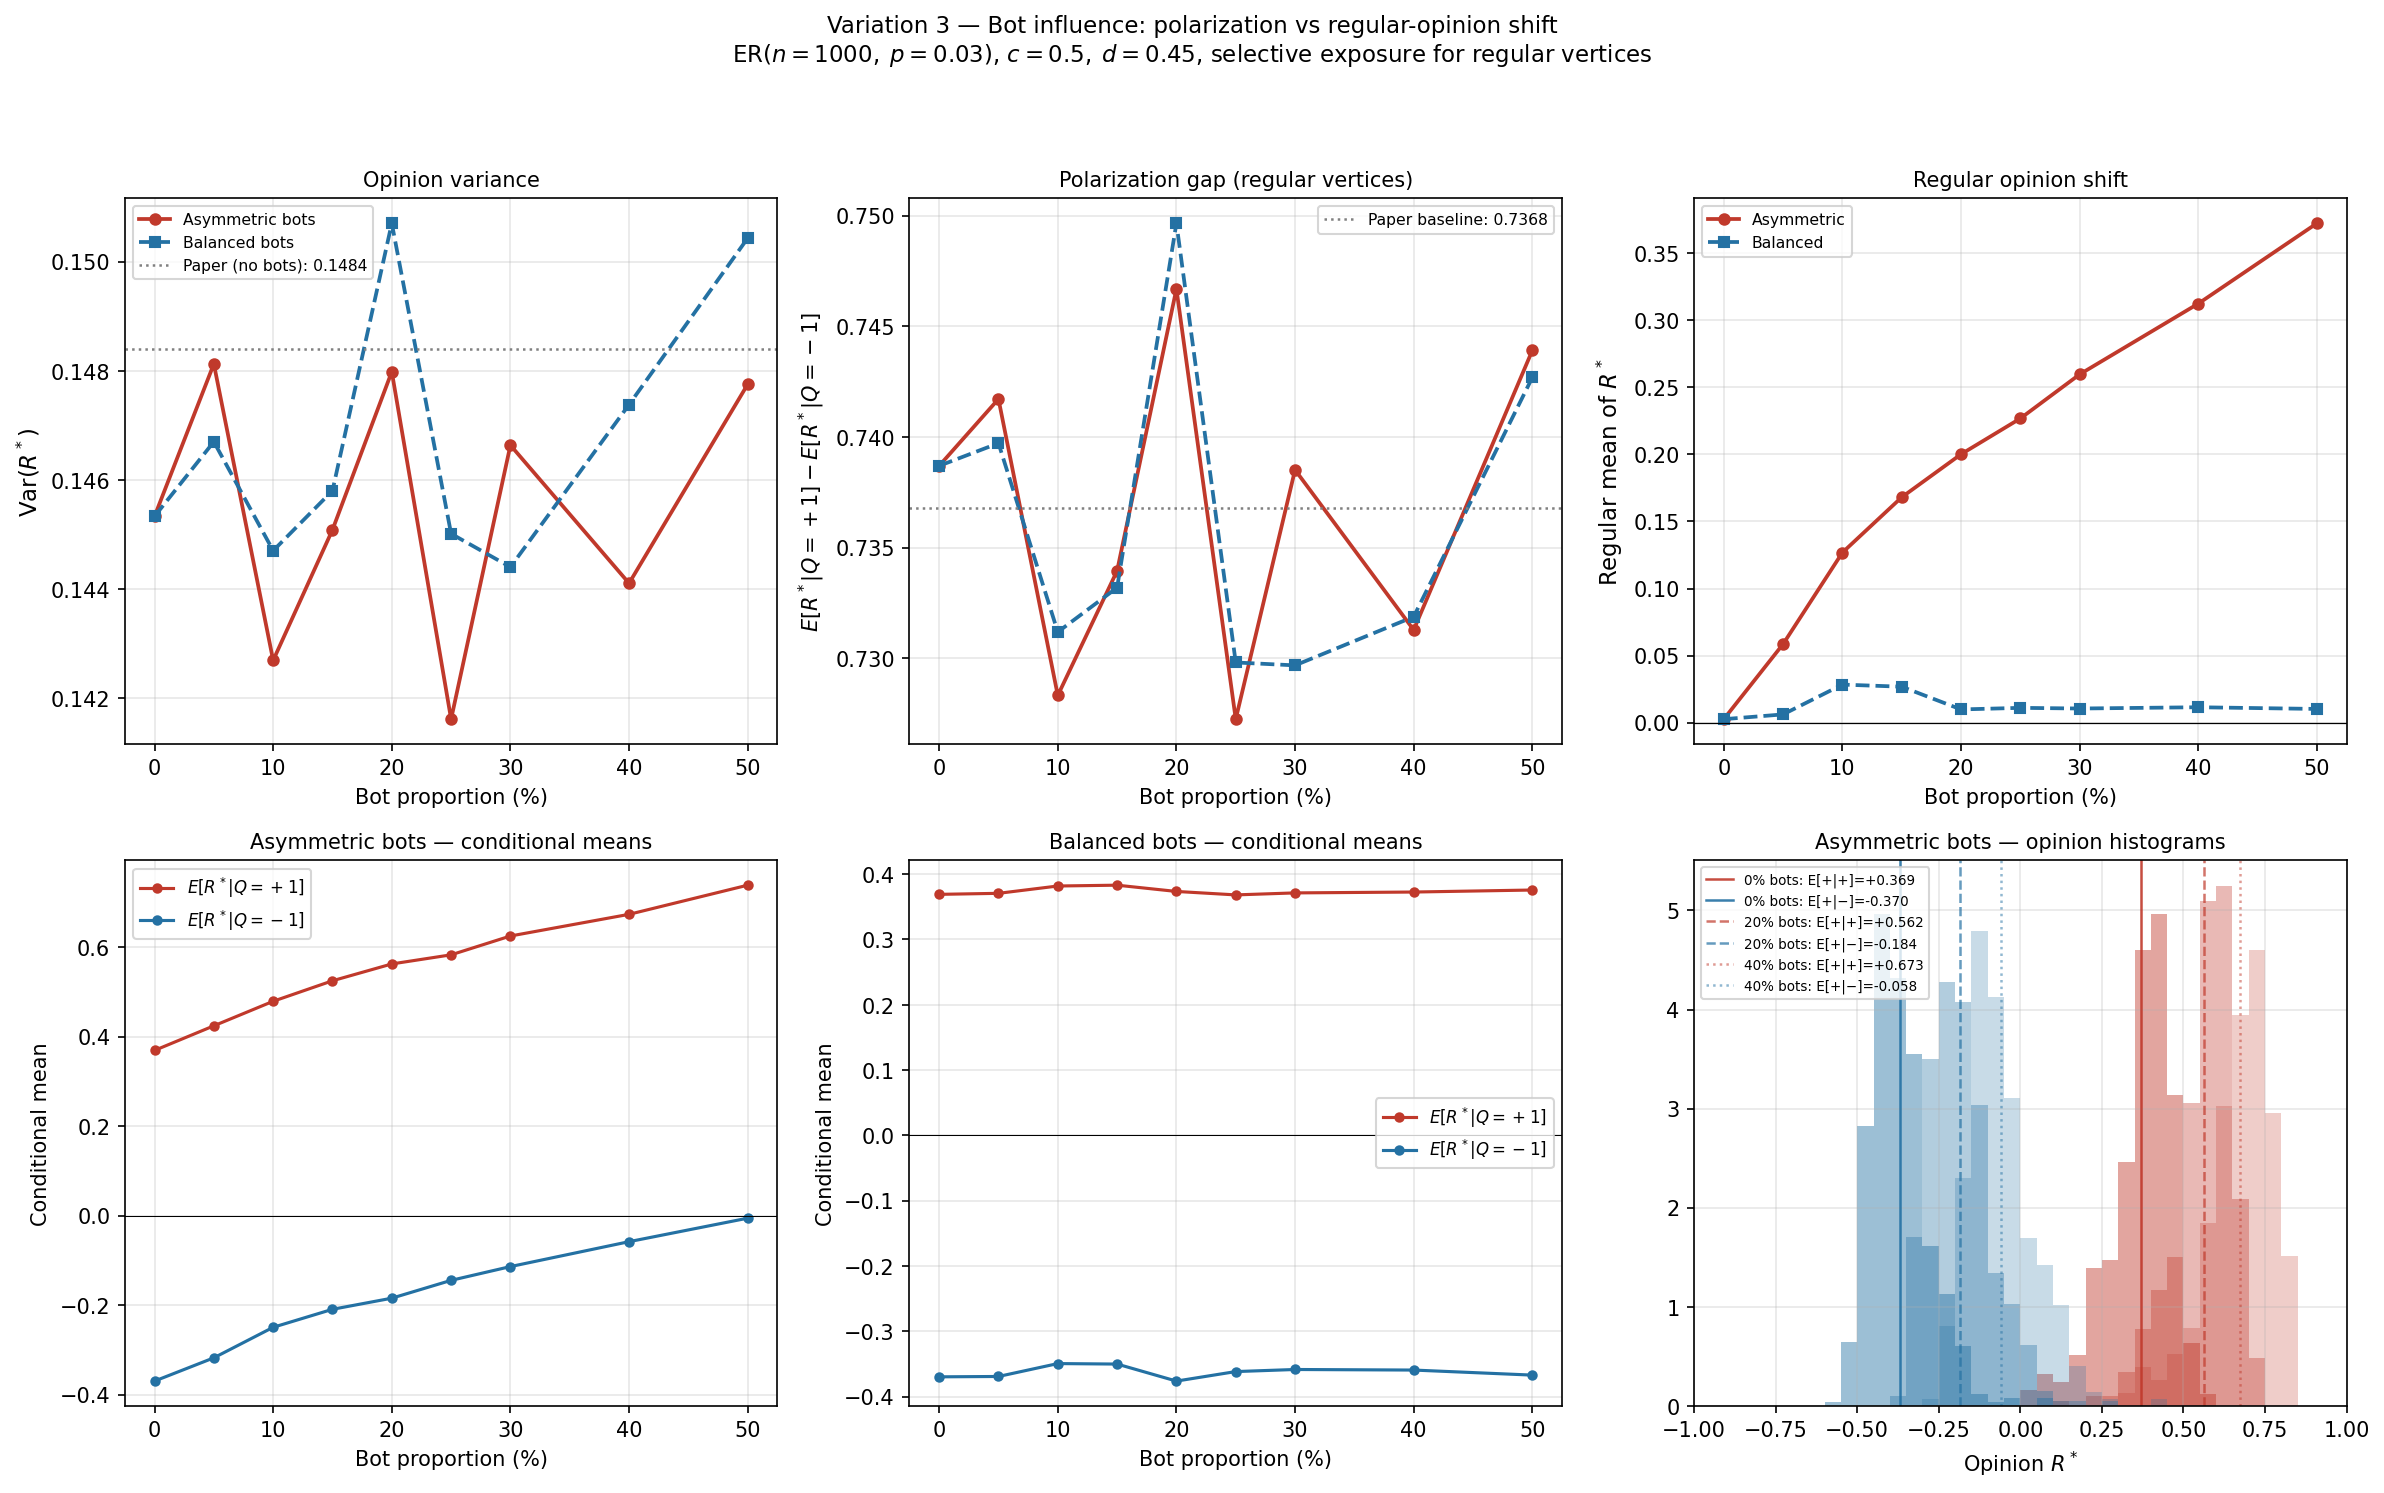
\includegraphics[width=0.9\textwidth]{variation3_bot_scan}
    \caption{Variation~3: bot influence scan.  Asymmetric bots shift the
    regular-agent mean, while the two-group polarization gap remains nearly
    constant.}
    \label{fig:variation3-bots}
\end{figure}

The variation therefore sharpens the interpretation of source-paper Figure~5.
Bots can move the population distribution, but in this implementation they do
not by themselves generate a much larger separation between $Q=+1$ and $Q=-1$
regular agents.

\subsection{Variation 4: Community Structure}

The fourth variation replaces random mixing with a two-block directed stochastic
block model.  The block sizes are $500$ and $500$, with within-block edge
probability $p_{\mathrm{in}}=0.05$ and cross-block probability
$p_{\mathrm{out}}=0.01$, giving a mean degree comparable to the ER baseline.
We tested both community-aligned attributes and randomly assigned attributes.
In the aligned case, $Q$ follows block membership with a small $2\%$ random
flip rate to avoid an exactly deterministic assignment.

Community structure matters only when it aligns with attributes.  With an SBM
echo chamber, the conditional means move to $0.5519$ and $-0.5465$, producing a
gap of $1.0984$ and variance $0.3137$.  The comparable ER graph with the same
community-aligned $Q$ vector has a gap of $0.7371$ and variance $0.1456$.  In
contrast, when $Q$ is randomly assigned across communities, the SBM gap is
$0.7385$, essentially the same as the ER random-$Q$ gap of $0.7328$.

\begin{figure}[t]
    \centering
    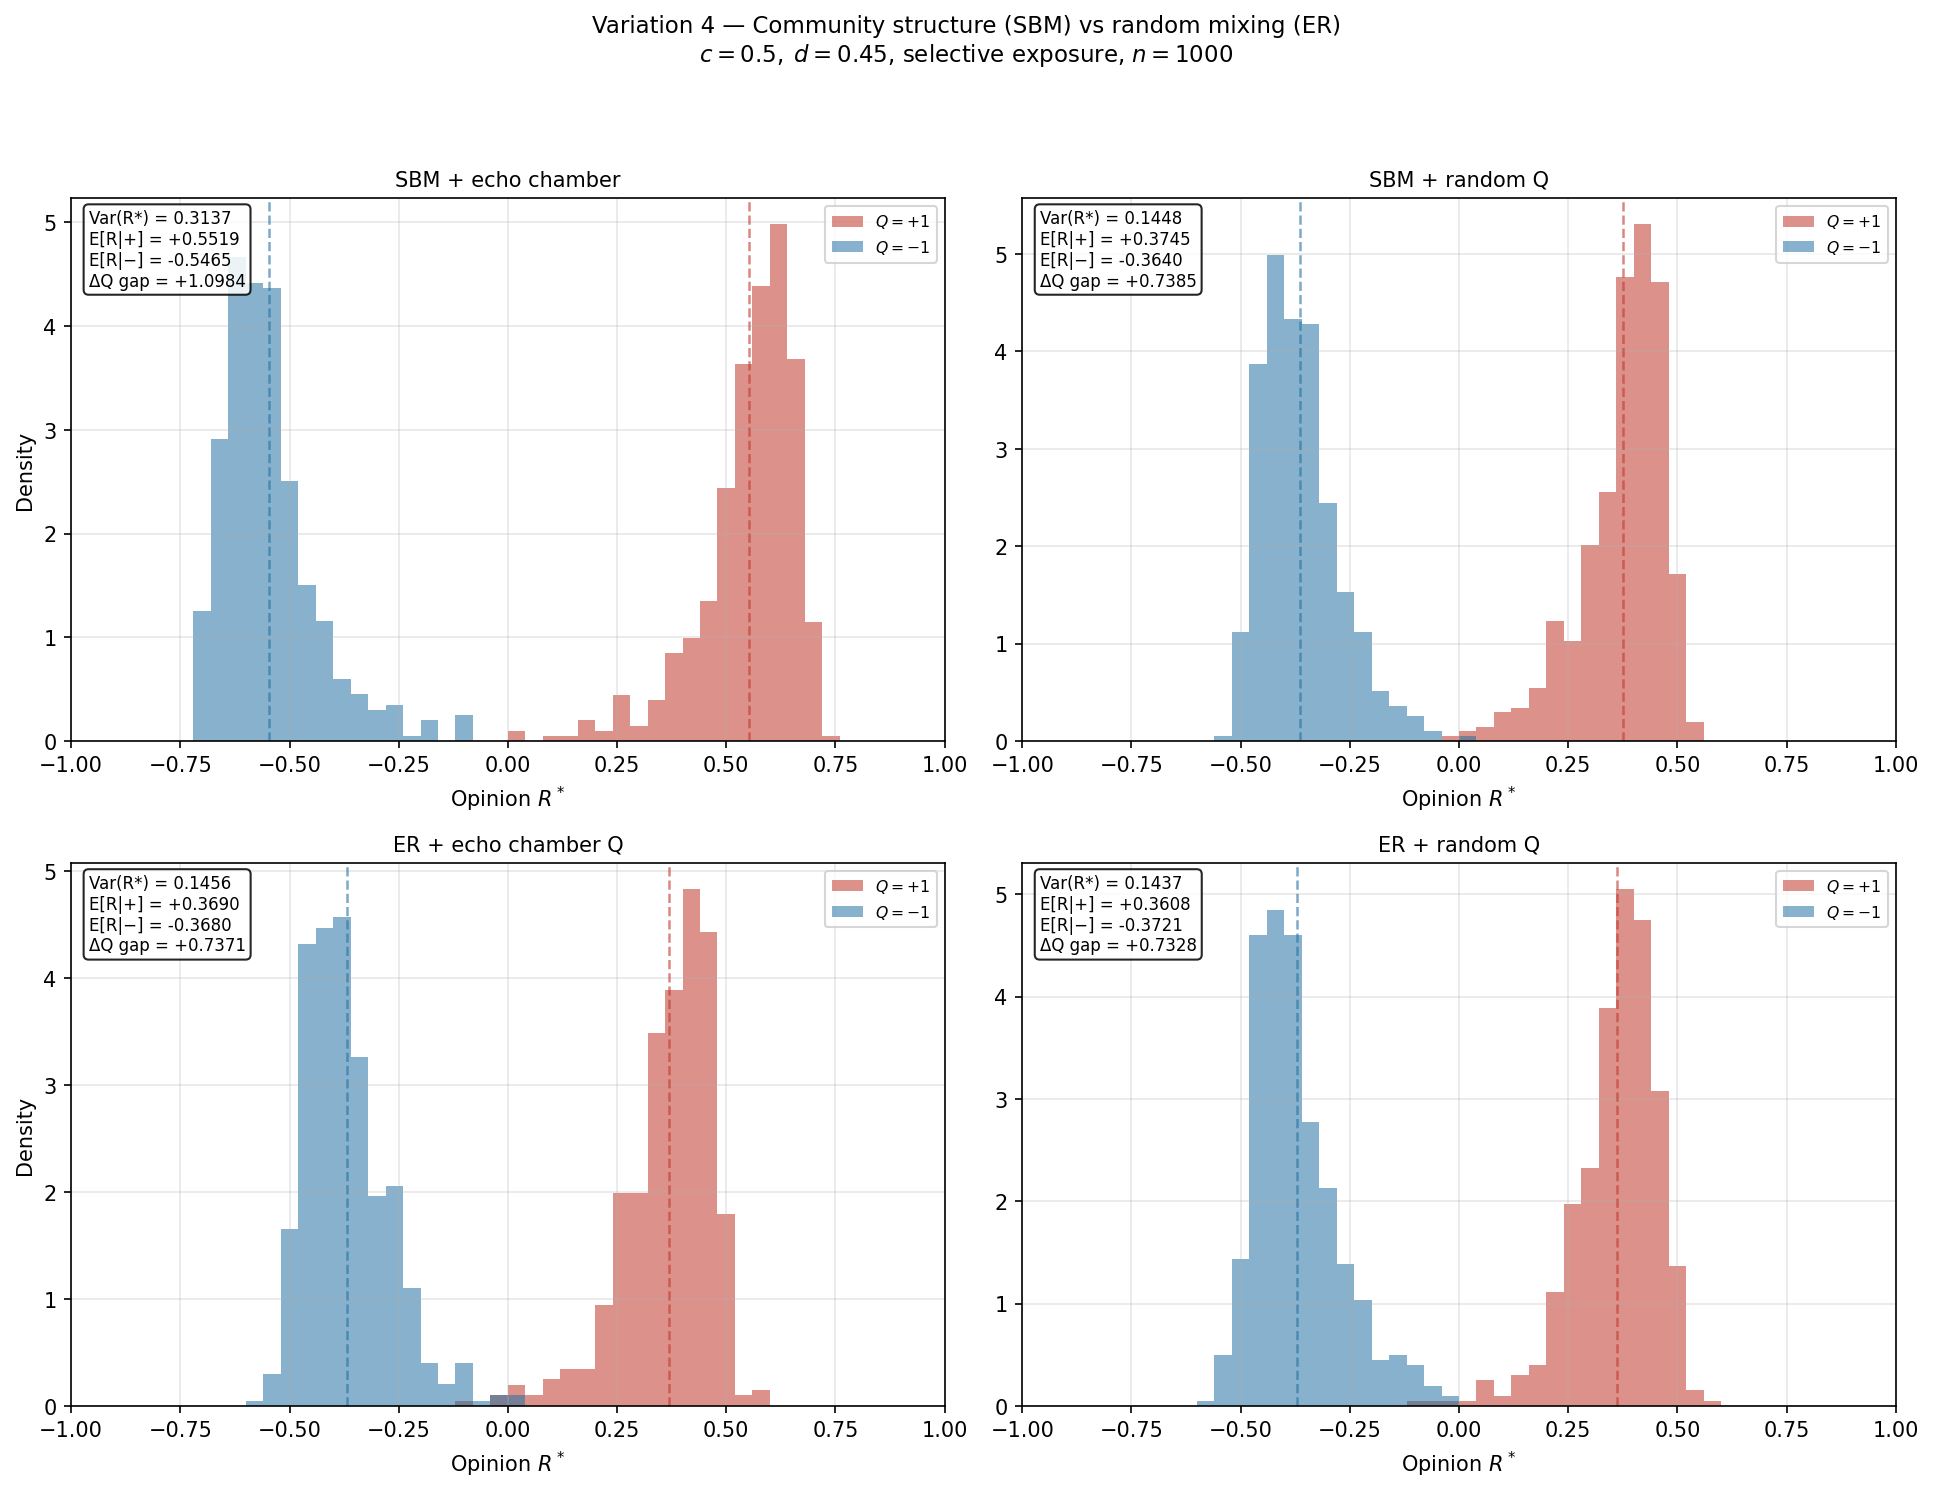
\includegraphics[width=0.9\textwidth]{variation4_community}
    \caption{Variation~4: community structure.  Modularity substantially
    amplifies polarization only when community membership aligns with the
    attribute that controls selective exposure.}
    \label{fig:variation4-community}
\end{figure}

This is the strongest extension beyond the original figures.  The source paper
explains selective exposure, but its ER simulations do not test how social
segregation and selective exposure interact.  Our SBM experiment suggests that
the same media mechanism can become much stronger when network communities and
attributes reinforce each other.

\section{Discussion}
\label{sec:discussion}

\subsection{What the Replication Supports}

The replication supports the central mathematical intuition of the source
paper.  When $d>0$, the update has a contraction component, and the effect of
the initial condition disappears.  When media exposure is common across agents,
network averaging tends to produce consensus-like distributions.  When media
signals are strongly conditioned on agent attributes and $d$ is large enough,
the stationary distribution separates into groups.  Memory reduces variance and
smooths trajectories, as predicted by the paper's comparison between memory and
no-memory processes.

The results also show that the paper's simulations are reproducible from the
published equations, even without author code.  The most important numerical
benchmark, source-paper Figure~4, is close to the reported values, and the
no-memory panel matches the applicable Proposition~4 finite-graph prediction.
This gives confidence that our implementation captures the intended recursion
rather than only producing visually similar plots.

\subsection{Scientific Critique}

Our main critique concerns the evidential scope of the simulations, not the
validity of the theorems.  The theoretical results apply to broad classes of
locally convergent directed random graphs, but the published simulation section
uses ER graphs for all main figures.  Our topology variation shows that
well-connected non-ER graphs can behave similarly, which is favorable to the
paper.  However, sparse graphs and community-aligned graphs can change the
variance and group separation substantially.  The paper's computational
evidence therefore supports the ER case more strongly than it supports broad
finite-network robustness.

A second critique concerns the interpretation of bots.  In our reproduction and
bot scan, asymmetric bots mainly translate the regular-agent distribution
toward the positive side.  They do not substantially increase the conditional
gap between the two regular groups.  Calling this outcome polarization can be
misleading unless polarization is defined broadly as distributional spread or
political displacement.  Under the group-separation criterion used in
source-paper Figure~4, the bot effect is better described as a directional
shift.

A third limitation is reproducibility detail.  The source paper states the
model and the main parameters clearly, but it does not report random seeds,
exact iteration counts, ensemble averages, or code.  These omissions do not
invalidate the results, because Theorem~1 gives a principled convergence
argument and our independent implementation recovers the key figures.  They do,
however, make exact figure matching harder and leave some visual differences
ambiguous.

\subsection{Limitations of Our Project}

Our own study also has limits.  Except for the ten-seed Figure~4 check, most
experiments are single-seed reproductions or parameter scans over one graph
size, so they should not be read as asymptotic empirical laws.  The power-law
configuration model removes
self-loops and multi-edges, which changes the realized degree distribution
relative to an unrestricted configuration model.  The community experiment uses
one two-block SBM design rather than a full modularity sweep.  These choices are
reasonable for a course replication, but a larger study should average over
many graph realizations and report confidence intervals.

\subsection{Reproducibility and AI Use}

The repository contains the Python source code, scripts for each figure, MATLAB
versions of the reproduced figure scripts, and dependency information.  The
generated figures are build artifacts that can be regenerated from the scripts.
The project used large language models as assistance for code drafting,
debugging suggestions, and language polishing.  The mathematical
interpretation, experimental design, script execution, and numerical claims in
this paper were checked against the code outputs by the team.

\section{Conclusion}
\label{sec:conclusion}

This project reproduced the directed-network opinion dynamics model of
Fraiman, Lin, and Olvera-Cravioto and tested it beyond the original ER
simulation setting.  The main qualitative results are recovered, and the
central polarization figure matches the paper closely in variance and
conditional means.  The robustness experiments show that selective exposure is
a stable mechanism, but its finite-network strength depends on topology,
low-degree structure, and especially alignment between network communities and
agent attributes.  Our final judgment is therefore balanced: the model is
mathematically convincing and computationally reproducible, while the original
simulation evidence is narrower than the range of graph settings covered by the
theory.

\addcontentsline{toc}{section}{References}
\begin{thebibliography}{9}

\bibitem{fraiman2024opinion}
Nicolas Fraiman, Tzu-Chi Lin, and Mariana Olvera-Cravioto.
\newblock Opinion dynamics on directed complex networks.
\newblock \emph{arXiv preprint arXiv:2209.00969v2}, 2024.

\bibitem{degroot1974reaching}
Morris H. DeGroot.
\newblock Reaching a consensus.
\newblock \emph{Journal of the American Statistical Association},
69(345):118--121, 1974.

\bibitem{friedkin1990social}
Noah E. Friedkin and Eugene C. Johnsen.
\newblock Social influence and opinions.
\newblock \emph{Journal of Mathematical Sociology}, 15(3--4):193--206, 1990.

\end{thebibliography}

\appendix

\section{Reproducibility Checklist}

Repository:
\url{https://github.com/PatrickEleeve/Network_Final}.

Environment:
\begin{quote}
\small
\begin{verbatim}
pip install -r requirements.txt
\end{verbatim}
\end{quote}
The required Python packages are NumPy, SciPy, and Matplotlib.

Core Python replications:
\begin{quote}
\small
\begin{verbatim}
python3 scripts/replicate_fig1_to_3.py
python3 scripts/replicate_fig4.py
python3 scripts/replicate_fig5.py
python3 scripts/replicate_fig6.py
python3 scripts/replicate_fig7.py
python3 scripts/validate_theorem1.py
\end{verbatim}
\end{quote}

Variation studies:
\begin{quote}
\small
\begin{verbatim}
python3 scripts/variation1_topology.py
python3 scripts/variation2_beta_scan.py
python3 scripts/variation3_bot_scan.py
python3 scripts/variation4_community.py
\end{verbatim}
\end{quote}

MATLAB figure scripts are stored in \texttt{matlab/}.  Running
\begin{quote}
\small
\begin{verbatim}
matlab/run_all_matlab_reproductions.m
\end{verbatim}
\end{quote}
regenerates the MATLAB versions of source-paper Figures~1--7.  Generated Python
figures are stored in \texttt{figures/}; MATLAB outputs are stored in
\texttt{figures\_matlab/}.

Main implementation assumptions are equal inbound-neighbor weights, documented
seed lists, independently sampled media signals at each time step, conservative
maximum iteration counts with a coupled-chain convergence diagnostic, and
independent implementation from the equations in the paper rather than from
author code.

\end{document}
